\documentclass[a4paper]{article}
\usepackage{fullpage}
\usepackage{amsmath}
\usepackage{amssymb}
\usepackage{breqn}
\usepackage{sectsty}
\usepackage{graphicx}
\usepackage{svg}
\usepackage{xcolor}
\usepackage{esint}
\usepackage{pdfpages}
\usepackage{fancyhdr}
\usepackage{chngcntr}
\usepackage{pagecolor}
\usepackage{caption}
\usepackage{subcaption}
\usepackage{physics}
\usepackage{float}
\counterwithin*{equation}{section}
\counterwithin*{equation}{subsection}
\renewcommand{\thesubsection}{\thesection.\alph{subsection}}
\renewcommand{\thesubsubsection}{\Roman{subsubsection}}
\newcommand{\horln}{\vspace{-6mm}\begin{flushleft}\mbox{}\hrulefill\mbox{}
	\end{flushleft}\vspace{-6mm}}
\newcommand\eq{\addtocounter{equation}{1}\tag{\theequation}}
\sectionfont{\huge}
\subsubsectionfont{\small}
\setlength{\parindent}{0cm}
\usepackage[citestyle=ieee]{biblatex}
\title{PHYS4123 GR Assignment 1}
\author{SID: 480344342}
\begin{document}
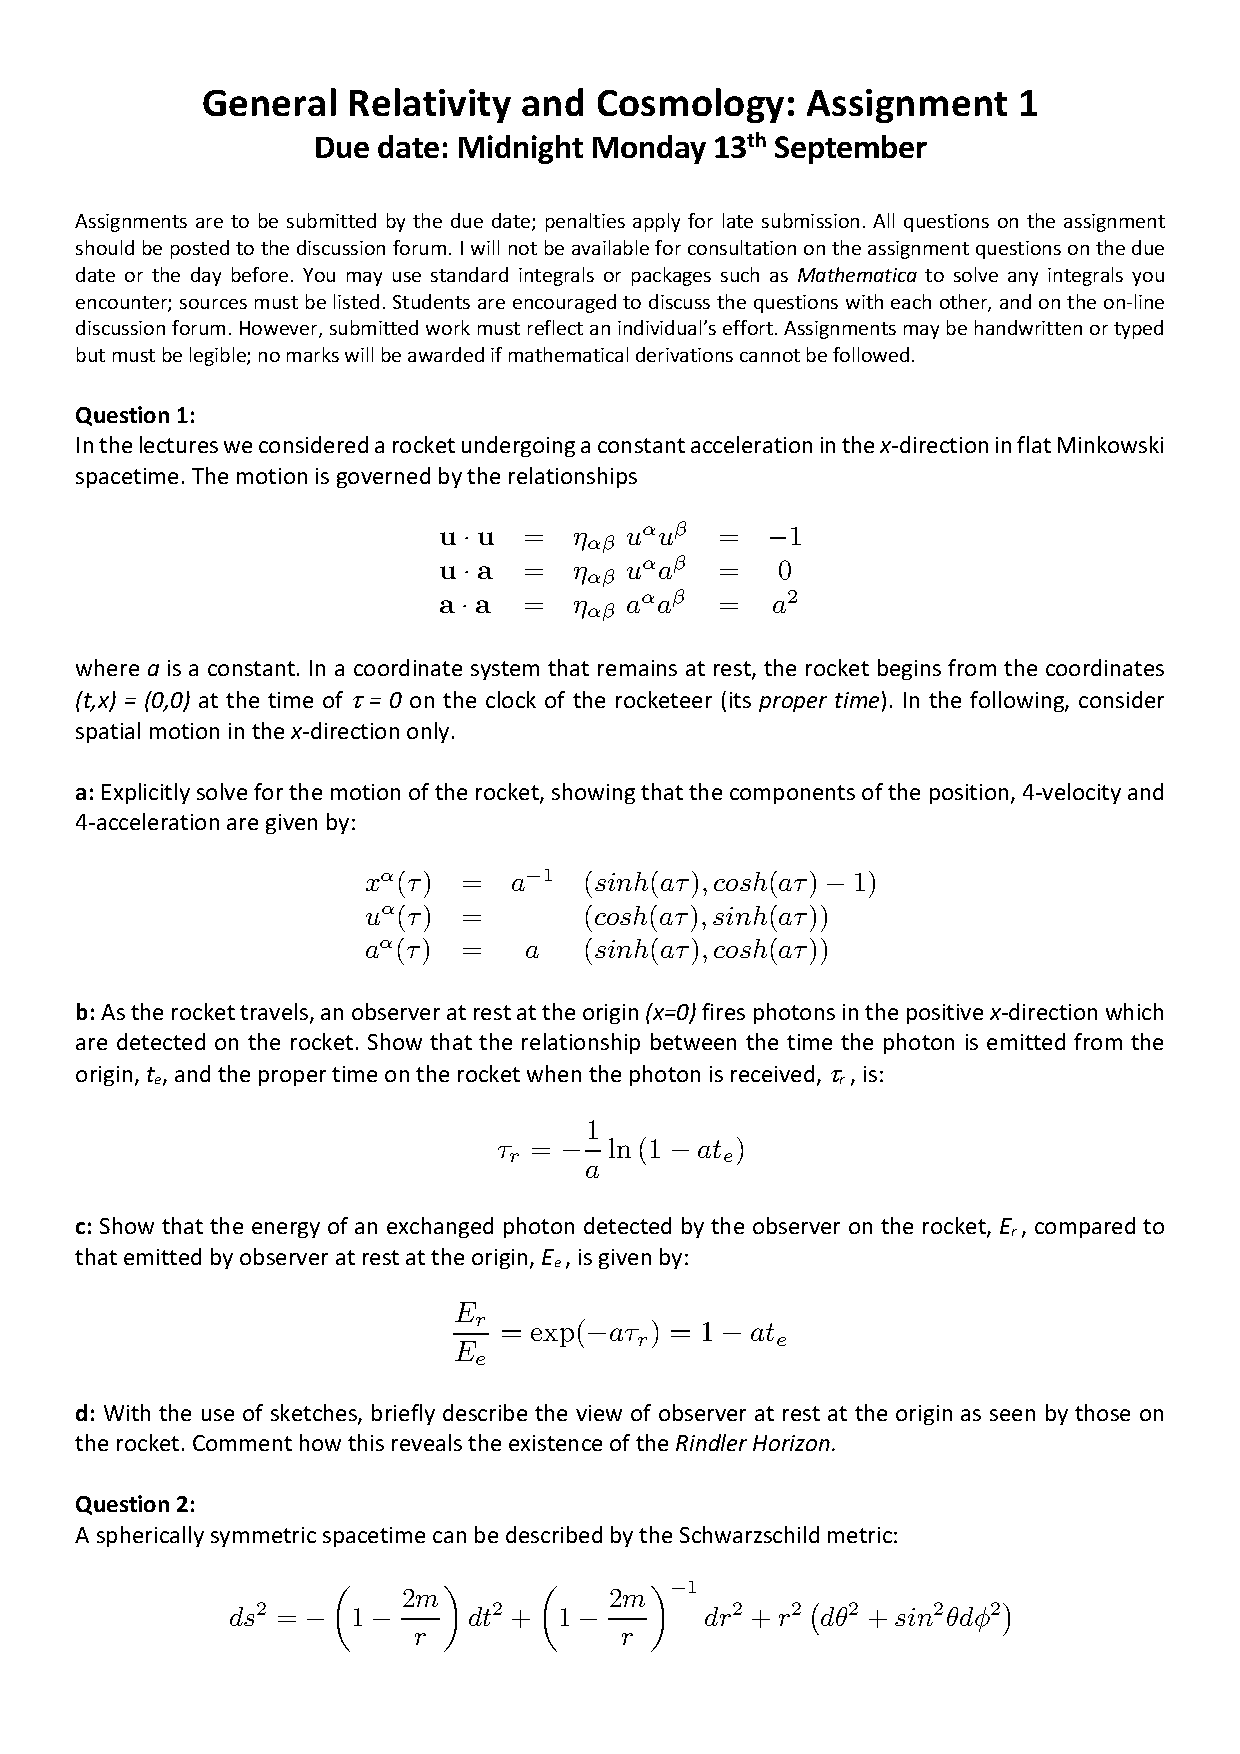
\includepdf[pages=-]{Figures/Questions}
\maketitle
\horln

\setcounter{page}{1}
\section{}
\subsubsection{}
Given:
\begin{align*}-1 &= \eta_{\alpha \beta} u^\alpha u^\beta\\
0 &= \eta_{\alpha \beta} u^\alpha a^\beta \\
a^2 &= \eta_{\alpha \beta} a^\alpha a^\beta
\end{align*}
Assuming spatial motion only occurs in $x^1$ gives:
\begin{align*}
-1 &= -u^0u^0 + u^1u^1\\
0 &= -u_0a_0 + u_1 a_1\\
a^2 &= -a^0a^0 + a^1a^1
\end{align*}
Then:
\begin{align*}
u^0u^0 &= u^1u^1 + 1 \eq \label{eq:1}\\
a_0 &= \frac{u_1}{u_0} a_1 \eq \label{eq:2}\\
a^1a^1 &= a^0a^0 + a^2 \eq \label{eq:3}
\end{align*}

Substituting \eqref{eq:2} into \eqref{eq:3}:
\begin{align*}
a^1a^1 &= a^2 \frac{1}{1-u^1u^1/u^0u^0}\\
a^0a^0 &= a^2 \frac{1}{u^0u^0/u^1u^1 - 1}
\end{align*}

Then using \eqref{eq:1}:
\begin{align*}
a^1a^1 &= a^2 (1 + u^1 u^1) = \left(\frac{du^1}{d\tau}\right)^2\\
a^0a^0 &=  a^2 (u^0 u^0 - 1) =  \left(\frac{du^0}{d\tau}\right)^2
\end{align*}

Integrating:
\begin{align*}
\tau &= \pm \int \frac{1}{\abs{a}\sqrt{1 + u^1 u^1}} du^1 = \pm \frac{1}{\abs{a}}\sinh^{-1}(u^1) + A\\
\tau &= \pm \int \frac{1}{\abs{a}\sqrt{u^0 u^0 - 1}} du^1 = \pm \frac{1}{\abs{a}}\cosh^{-1}(u^0) + B
\end{align*}
Assuming $u^0 > 0$. Since the rocket begins at rest, $(u^0, u^1) = (1, 0)$ at $\tau = 0$ and$C = 0$ and $B = 0$. Also, letting $\mp \abs{a} = a$ (such that the sign of $a$ is the direction of $a^1$):
\begin{align*}
(u^0, u^1) &= (\cosh(a \tau), \sinh(a\tau))
\end{align*}
Differentiating gives:
\begin{align*}
	(a^0, a^1) &= a(\sinh(a \tau), \cosh(a\tau))
\end{align*}
Whereas integrating gives:
\begin{align*}
	(x^0, x^1) &= \frac{1}{a}(\sinh(a \tau) + C, \cosh(a\tau) + D)
\end{align*}
Where the initial conditions $(x^0, x^1) = (0, 0)$ at $\tau = 0$ constrain $C = 0$ and $D = -1$.
% \begin{figure}[H]
%    { \centering
%         \includesvg[width=0.98\textwidth]{Figures/OtherMetals.svg}
%         \caption{\textbf{Valid excitation angles for SPP excitation by four-wave mixing at various metal-dielectric interfaces.} The valid angles depend very little on the type of metal used in the interface. This is especially true when both of the angles are not glancing (not close to $90^\circ$), and is because the wavevector of the SPP does not depend strongly on the relative permittivity of the metal ($k'_i = \frac{\omega'_i}{c} \sqrt{\varepsilon(\omega'_i)}/\sqrt{\varepsilon(\omega'_i)+1}$), where the fraction is close to $1$ since $\varepsilon \gg 1$ (and frequencies do not change with refractive index or relative permittivity).}
%     \label{fig:2}}
% \subsubsection{}
%     {\centering
%         \includesvg[width=0.98\textwidth]{Figures/Au_H20.svg}
%         \caption{\textbf{Valid angles for SPP excitation at an interface between water and gold.} Comparing to Fig. 1, the valid angles have changed significantly, particularly at glancing angles. This is because the real part of the wavevector of the SPP (e.g. $\pm\Re(k'_1) = 2k_1 \sin(\theta_1) - k_2 \sin(\theta_2)$) depends \textit{linearly} on the index of the dielectric ($k = k_0 n$). Comparing to Fig. 2, the index of the dielectric (which strongly changes $\Re(k'_i)$) therefore has a much stronger effect on the valid angles than the $\varepsilon$ of the metal (which weakly changes $k'_i$).}
%     \label{fig:3}}
% \end{figure}

% \includepdf[pages=-]{Plasmonics.pdf}

\end{document}
